\section{The RationalGRL Tool}
\label{sect:tool}
\todo{Marc}{Marc}{Currently this section comes from my thesis where I present the tool as future work. Here we should explain it}

GRL has a well-documented and well-maintained tool called jUCMNav~\cite{jUCMNav}. This tool is an extension to Eclipse. Although it is a rich tool with many features, we also believe it is not very easy to set it up. This seriously harms the exposure of the language, as well as the ability for practitioners to use it. We have started to implement a simple version of GRL as an online tool in Javascript. This makes it usable from the browser, without requiring the installation of any tool. The tool can be used from the following address:

\begin{quote}
\url{http://marcvanzee.nl/RationalGRL/editor}
\end{quote}

A screenshot of the tool is shown in Figure~\ref{fig:goalmodeling:tool}. As shown, there are two tabs in the tool, one for ``Argument'' and one for ``GRL''. The argument part has not been implemented yet, and the GRL part only partly, but the idea behind the tool should be clear. Users are able to work on argumentation and on goal modeling in parallel, where the argumentation consists of forming arguments and counterarguments by instantiating argument schemes and answering critical questions. 

\begin{figure*}[h!]
\centering
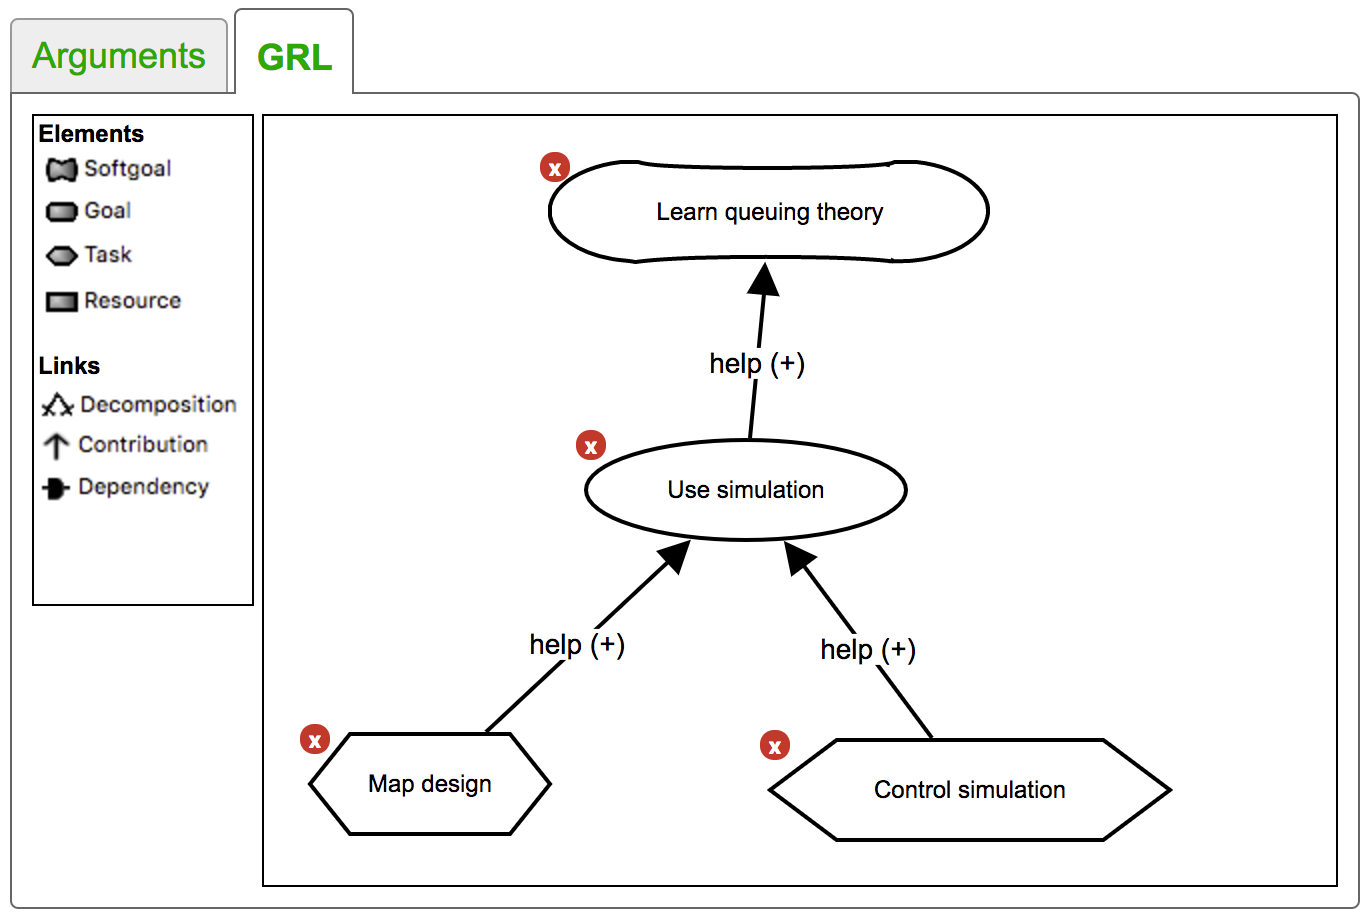
\includegraphics[scale=0.5]{img/tool_screen}
\caption{Screenshot of the prototype tool}
\label{fig:goalmodeling:tool}
\end{figure*}

An important aspect of the tool is that users can switch freely between these two ways of modeling the problem. One can model the entire problem in GRL, or one can do everything using argumentation. However, we believe the most powerful way to do so is to switch back and forth. For instance, one can create a simple goal model in GRL, and then turn to the argumentation part, which the users can look at the various critical questions for the elements, which may trigger discussions. These discussions results in new arguments for and against the elements in the goal model. Once this process is completed, one may switch to the goal model again, and so on. We believe that in this way, there is a close and natural coupling between modeling the goals of an organization as well as rationalizing them with arguments.